\documentclass[12pt, a4paper]{article}
\usepackage[utf8]{inputenc}
\usepackage{answers}
\usepackage{setspace}
\usepackage{graphicx}
\usepackage{subfigure}
\usepackage{lipsum}
\usepackage{wrapfig}
\usepackage{parskip}
\usepackage{multicol}
\usepackage{hyperref}
\usepackage{enumerate}
\setlength{\parindent}{0cm}
\usepackage[left=3.00cm, right=1.50cm, top=3.00cm, bottom=1.50cm]{geometry} 
\usepackage{amsmath,amsthm,amssymb}
\usepackage[spanish]{babel}
\usepackage{listings}
\usepackage{multirow}
\usepackage{lscape}
\usepackage[toc,page]{appendix}
\selectlanguage{spanish}

\begin{document}
 
 
\title{ Medición con Elementos Finitos \\ “Ensayo de fatiga de Asfalto” }
\author{PAPPALARDO, Leonardo \\ RONCONI, Jorge E.}
 
\maketitle

\section{Introduccion}
		
En el siguiente informe se muestra una reproduccion del trabajo "Life cycle analysis of pavement overlays made with Engineered Cementitious Composites", publicado en el año 2013, por Qian, Li, Zhang, Keoleian,  donde analizan la la vida util de la rehabilitacion de caminos de hormigon con asfalto.

Para esto, se desarrolo un modelo por el Metodo de los Elementos Finitos, en el cual se ensayo a traccion una "probeta de asfalto", con condiciones comparables a las propuesta en el trabajo antes citado, con la finalidad de comparar los resultados.

\begin{figure}[h]
	\centering
	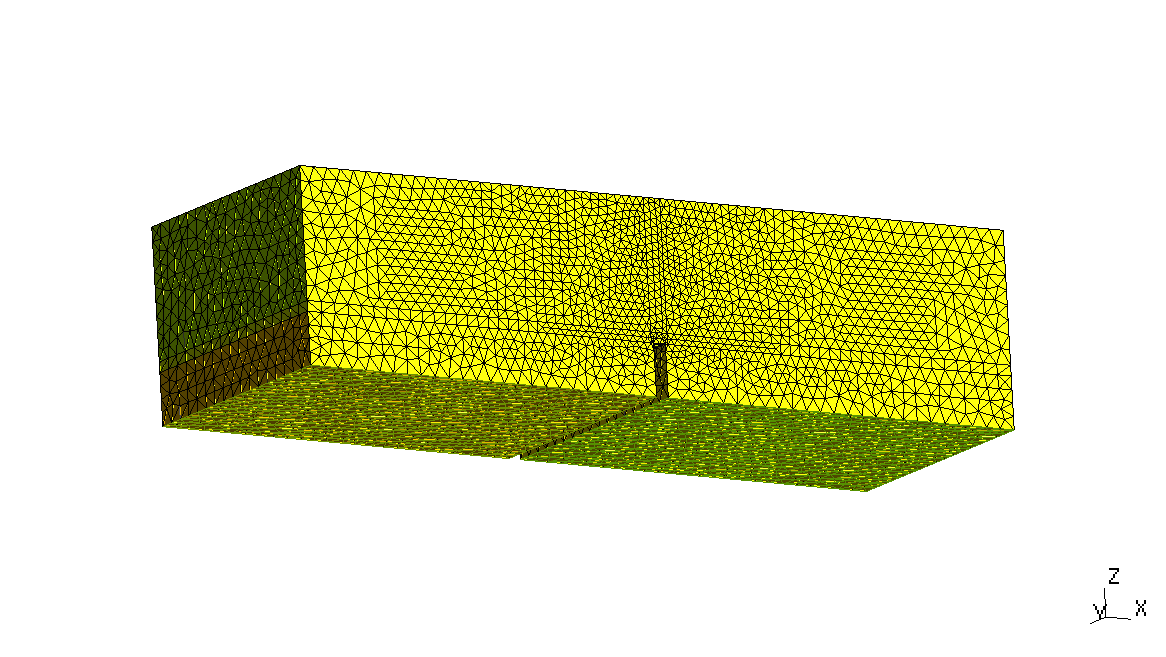
\includegraphics[width=0.7\textwidth]{img/modelo.png}
	\caption{Probeta a ensayar}
	\label{fig:modelo}
\end{figure}

En una intecion de optimisar el comportamiento, se propone adherir entre capas, un geotextil que funciones como elemento que tome las tracciones en lugar del asfalto.

\section{Formulacion variacional}
Las ecuaciones que gobiernan las deformaciones elásticas pequeñas de un cuerpo “$\Omega$” pueden ser escritas como se muestra en la expresion \ref{equ:defelas}:

\begin{subequations}
	\begin{equation}
		- \nabla \cdot \sigma  = f  \quad \quad \quad en \, \Omega
		\label{equ:defelas-a}
	\end{equation}
	\begin{equation}
		\sigma  = \lambda \cdot tr(\epsilon) \cdot I + 2 \cdot \mu \cdot \epsilon \quad \quad en \, \Omega
		\label{equ:defelas-b}
	\end{equation}
	\begin{equation}
		\epsilon  = \frac{1}{2} \cdot (\nabla u + (\nabla u)^t) \quad \quad en \, \Omega
		\label{equ:defelas-c}
	\end{equation}
	\label{equ:defelas}
\end{subequations}

Donde:
\begin{itemize}
	\item $\sigma$: es el tensor de tensiones
	\item $f$: es la fuerza de cuerpo por unidad de volumen.
	\item $\lambda y \mu]$: son los parámetros de elasticidad de Lamé del material en $\Omega$.
	\item $I$: es el tensor indentidad.
	\item $tr$: es el operador traza de un tensor
	\item $\epsilon$: es el tensor de deformación unitaria simétrico (gradiente simétrico)
	\item $u$: es el campo vectorial de desplazamientos. 
\end{itemize}

Cuando hablamos de una integracion en el tiempo, ya que este modelo es un ensayo elastodinamico, en lugar de usar la expresion \ref{equ:defelas-a}, se usa la \ref{equ:momenolineal}, donde se plantea el equilibrio del momento lineal.

\begin{equation}
	\nabla \cdot \sigma+ \rho b = \rho \ddot{u}
	\label{equ:momenolineal}
\end{equation}

En donde $u$ es el campo vectorial de desplazamiento, $\ddot{u}$ es la aceleración, $\rho$ la densidad del material, $b$ una fuerza en la masa.

La forma débil se obtiene fácilmente integrando por partes la ecuación de equilibrio mediante una función de prueba $v \in V$ siendo $V$ un espacio de función adecuado que satisface las condiciones límite de desplazamiento:

\begin{equation}
	\int_{\Omega} \rho \ddot{u} \cdot v \,dx + \int_{\Omega} \sigma(u):\epsilon(v) \, dx = \int_{\Omega} \rho b \cdot v \, dx + \int_{\delta \Omega} (\sigma \cdot n) \cdot v \, ds \quad \quad \forall v \in V
	\label{equ:defelas-com}
\end{equation}

Se pueden introducir términos disipativos a nivel de la ecuación constitutiva si estos mecanismos son bien conocidos, pero con bastante frecuencia no es así. La disipación puede entonces modelarse añadiendo a la ecuación de evolución anterior un término de amortiguación en función de la velocidad $ \dot{u} $

Cuando se sabe poco sobre el origen de la amortiguación en la estructura, una elección popular para la matriz de amortiguación, conocida como amortiguación de Rayleigh, consiste en utilizar una combinación lineal de la matriz de masa y rigidez $[C]= \nu_M [M]+ \nu_K [K]$ con dos parámetros positivos $\nu_M$ $\nu_K$ que se pueden ajustar a las medidas experimentales.

\subsection{Discretizacion del Tiempo}

Ahora introducimos una discretización de tiempo del estudio del intervalo $[0;T]$ en incrementos de tiempo $N+1$ $t_0=0,t_1,...,t_N,t_{N+1}=T$ con $\Delta t=\frac{T}{N}$ que denota el paso de tiempo (supuesto constante). La resolución hará uso del método generalizado-$\alpha$ que puede ser visto como una extensión del ampliamente utilizado método de Newmark-$\beta$. Como método implícito, es incondicionalmente estable para una elección adecuada de los coeficientes, de modo que se pueden utilizar pasos de tiempo bastante grandes. También ofrece una precisión de segundo orden.

El método consiste en resolver la ecuación de evolución dinámica en un tiempo intermedio entre $t_N$ y $t_{N+1}$, de la siguiente manera

\begin{equation}
	[M](\ddot{u}_{n+1-\alpha_m})+[C](\dot{u}_{n+1-\alpha_f})+[K](u_{n+1-\alpha_m})=F(t_{n+1-\alpha_m})
\end{equation}

Con las siguientes aproximaciones:

\begin{equation}
	u_{n+1} = u_n + \Delta t(\dot{u}_n) + \frac{\Delta t^2}{2}((1-2\beta)\ddot{u}_n + 2 \beta \ddot{u}_{n+1})
	\dot{u}_{n+1} = \dot{u}_n + \Delta t((1- \gamma )\ddot{u}_n) + \gamma \ddot{u}_{n+1})
\end{equation}

\section{Procedimiento}

Todo el codigo del proyecto se encuentra subido a GitHub: \url{https://github.com/driendro/fatiga_asfalto_fem}

Se utilizo un script realizado con Python 3, en donde, con la libreria \textbf{pygmsh} definimos la geometría de la pieza en 3D, a través de una funcion, lo que nos permite, variar facilmente los parametros de la geometria de la probeta. Luego, utilizando el mashador de GMSH, obtenemos un mallado de la superficie y el volumen. Por ultimo, luego de convertir la masha a xml usando \textbf{dolfin-convert}, con el fin de que "FEniCS" pueda interpretar los nodos y etiquetas de los diferentes volumenes y superficies.

\subsubsection{Codigo}

El script de Python consta de 2 archivos, el primero esta definida la funcion que diseña la geometria, usando pygmsh, el segundo es el script, que desarrolla el calculo en si.

\paragraph{geometria.py} Este archivo se divide en las siguientes partes:

\begin{enumerate}
	\item Deficiones de la geometria de la probeta, tomadas de los parametros de la funcion
	\item Puntos de que definen la geometria
	\item Lineas, bordes, superficies y volumenes definidos.
	\item definimos los valores fisicos del volumen y la superficie.
	\item creamos la malla y el xml, con la informacion para FEniCS. 
\end{enumerate}

Cabe aclarar que en la zona central, se dimensiona un sector al cual se le puede aumentar la densidad de puntos para un mejor detallado de la informacion.

\paragraph{calculo.py} Este archivo cuenta con la logica del procesamiento de la simulacion:

\begin{enumerate}
	\item Parametros dimensionales de la geometria (tamaños y espesores)
	\item Compara para no regenerar la malla siempre.
	\item Clases que definene las propiedades de los materiales para cada parte de la probeta
	\item Parametros de Elasticidad y coeficiente de Poisson.
	\item Clases que definenen las funciones de calculo, y por ultimo el calculo por EF. 
\end{enumerate}


En el modelo geometrico, se definieron 4 volumenes (Figura \ref{fig:vol}) y 2 superficies (bordes) (Figura \ref{fig:bord}), las cuales tendran las condiciones de borde para la simulacion.

\begin{figure}[h]
	\centering
	\subfigure[Volumenes]{\label{fig:vol} 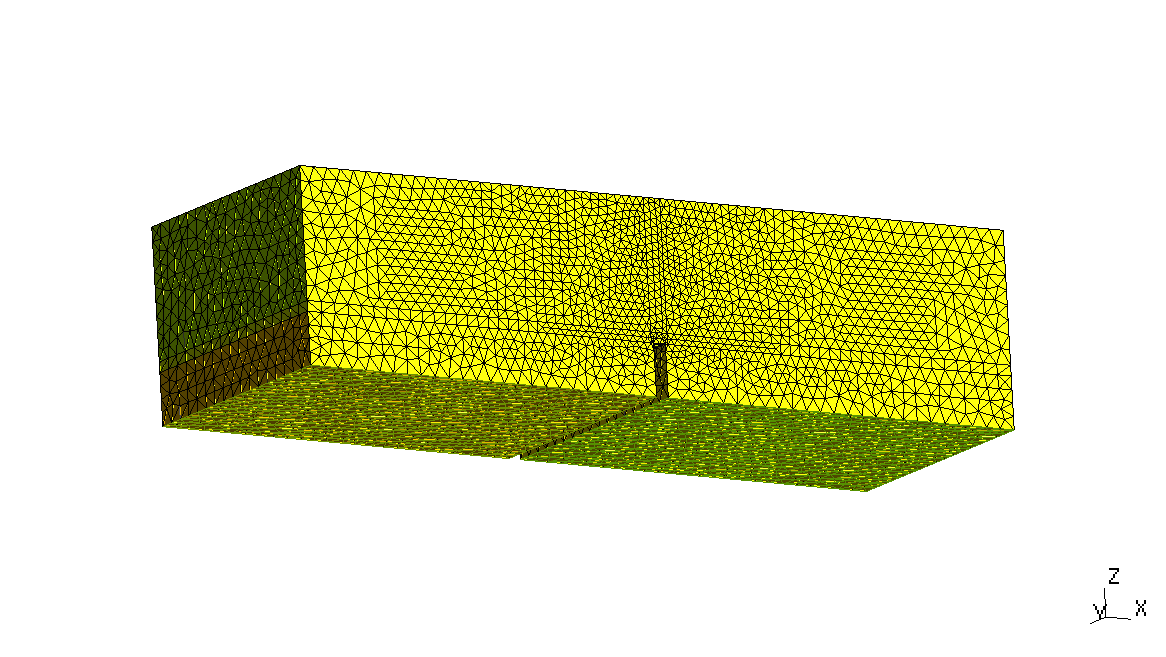
\includegraphics[width=0.4\textwidth]{img/modelo.png}}
	\subfigure[Bordes]{\label{fig:bord} 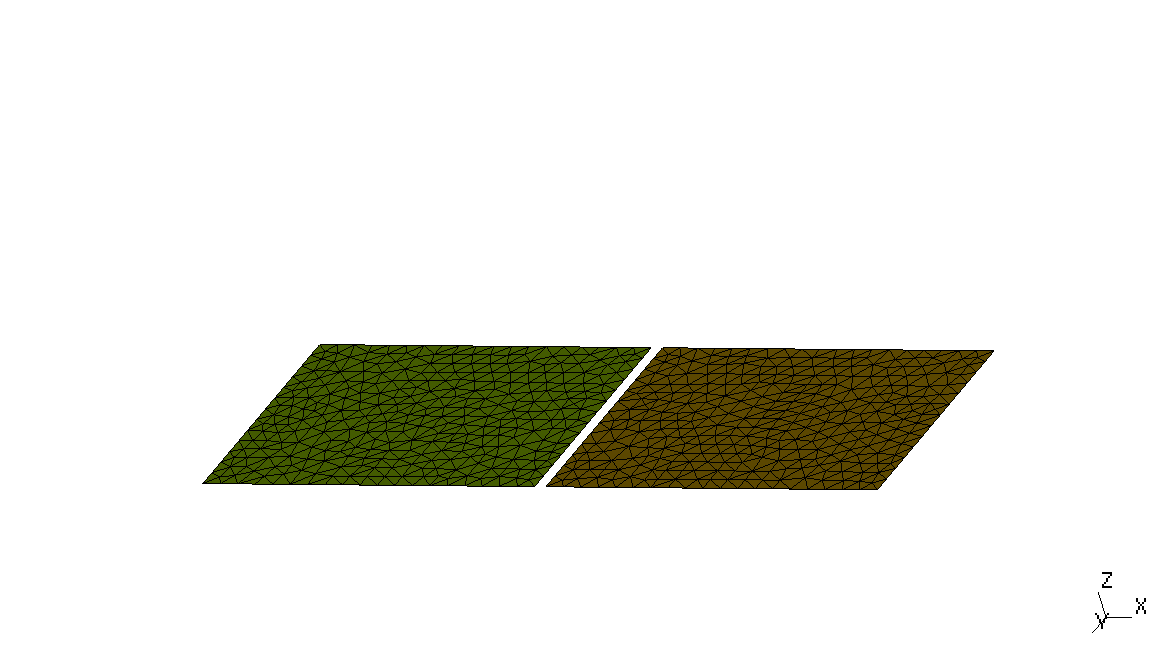
\includegraphics[width=0.4\textwidth]{img/modelo_sup.png}}
	\caption{Modelo} \label{fig:modelo1}
\end{figure}

Las propiedades del los materiales se muestran en la tabla \ref{tab:mat1}:

\begin{table}[]
	\centering
	\resizebox{0.7\textwidth}{!}{%
	\begin{tabular}{|l|l|l|l|}
	\hline
	Volumen & Material & E {[}MPa{]} & $\nu$ \\ \hline
	1		& Asfalto   &  1000 & 0,35 \\ \hline
	2		& Geotextil & 10000 & 0,30 \\ \hline
	3 y 4	& Hormigon  & 20000 & 0,20 \\ \hline
	\end{tabular}%
	}
	\caption{Propiedades de los materiales}
	\label{tab:mat1}
\end{table}

\subsection{Simulacion 1}

En la primera modelacion, se intento reproducir las consiciones del trabajo previamente realizado, por lo que, las propiedades del material son las del Hormigon.

En lo referente a las condicones de borde, todas las superficies del modelo se encuentran libres, salvo las mostradas en la figura \ref{fig:bord}, en este caso, el borde de la derecha se encuentra sujeto ($desplazamiento=0$), y el de la izquierda es cargado con una fuerza equivalente al E del Hormigon (Expresion \ref{equ:fuerza_1}), hacia la derecha, separando las bases inferiores.

\begin{equation}
	\left\{\begin{matrix}
		p=p \cdot \frac{t}{tc} & 0<t<tc \\ 
		p=0 & tc<t<T
		\end{matrix}
		\right.
	\label{equ:fuerza_1}
\end{equation}

Donde:
\begin{itemize}
	\item T: Tiempo relativo del ensayo.
	\item tc: Tiempo de corte.
	\item pc: Valor de la fuerza maxima
\end{itemize}

Luego de correr la simulacion (Imagen \ref{fig:sim1}), se observa una consentracion de tensiones de tracciones, en el plano donde termina la endidura, y compresiones en la cara superior, respondiendo a una flexion. estos resultados se contrastan correctamente con los obtenidos en el trabajo original \ref{fig:real}, incluso ellos muestran como se fisura y se despega el bloque superior en un plano a la altura de la endidura.

\begin{figure}[h]
	\centering
	\subfigure[t=$10$; T=$20$; Pc=$\frac{E}{2000}$]{\label{fig:sim1} 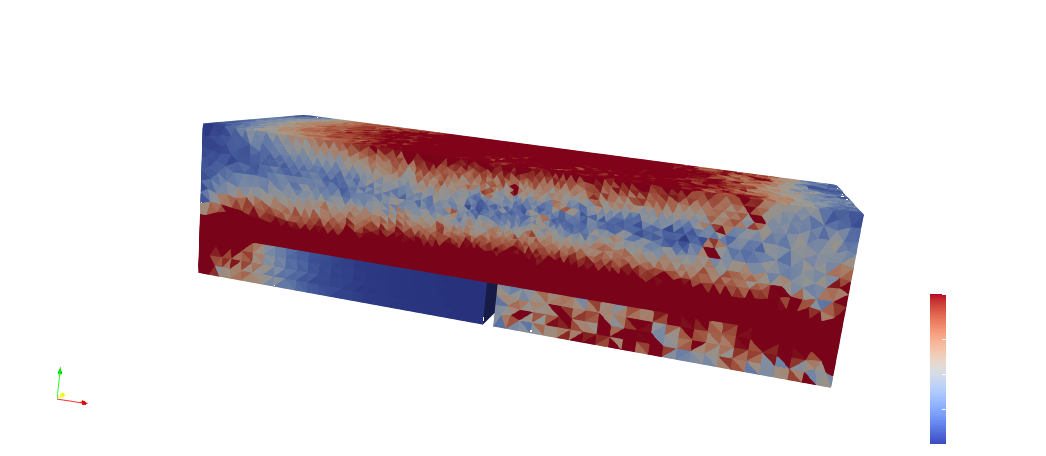
\includegraphics[width=0.45\textwidth]{img/1/tensiones.png}}
	\subfigure[Foto del trabajo original]{\label{fig:real} 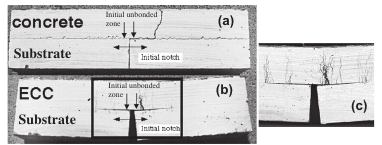
\includegraphics[width=0.45\textwidth]{img/1/ensayo.png}}
	\caption{Simulacion 1}
\end{figure}


\end{document}
